
\section{Introduction}

\begin{frame}
 	\begin{center}
 	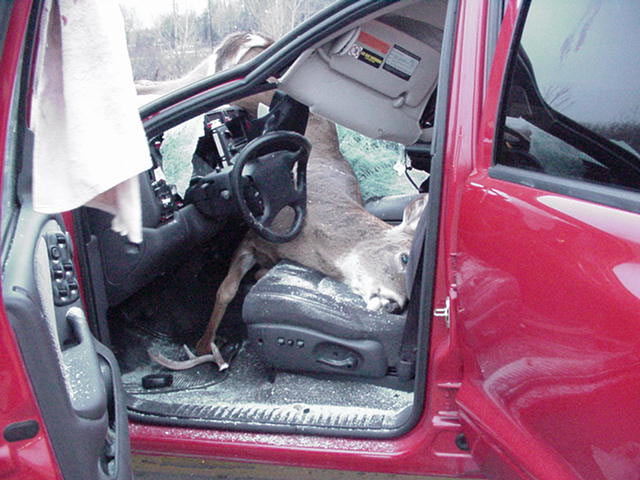
\includegraphics[height=7cm]{DeervsDurango}
 	\end{center}
\end{frame}

\begin{frame}
    \frametitle{Background}
In the U.S., between July 1, 2011 and June 30, 2012:
    \begin{itemize}
    	\item 1.23 million deer-vehicle collisions occurred.
    	\item Costs are more than \$4 billion in vehicle damage.
    	\item The average claim for deer-vehicle collisions was \$3,305 per accident.
    	\item The Insurance Institute for Highway Safety (IIHS) noted that deer-vehicle collisions in the U.S. cause about 200 fatalities annually.
    \end{itemize}
\emph{(State Farm, Insurance Journal)}
\end{frame}


\begin{frame}
    \frametitle{Question?}
How do insurance companies manage funds associated with deer vehicle collisions?
\end{frame}


\section{Population Biology}

\begin{frame}
    \frametitle{Deer Population}
    \begin{itemize}
    	\item Assumptions
		\begin{itemize}
    		\item Population is near carrying capacity.
    		\item The only predation is human i.e. hunting and car fatalities.
    		\item Migrations rates are balanced across counties.
		\item Customers of one insurance company experience the same collision rate as the general population.
    		\end{itemize}
    \end{itemize}
\end{frame}

\begin{frame}
    \frametitle{Logistic Equation with Harvest}
	\vspace{-1cm}
	\begin{eqnarray*}
		\frac{dx}{dt} &=& rx \left( 1-\frac{x}{f} \right) -hx
	\end{eqnarray*}
	\begin{itemize}
		\item $f$ - Carrying capacity
		\item $r$ - Growth rate
		\item $h$ - Harvest rate
	\end{itemize}
\end{frame}

\begin{frame}
    \frametitle{Rescaling the Logistic Equation with Harvest}
	\vspace{-1cm}
	\begin{eqnarray*}
		\frac{dx}{dt} &=& rx \left( 1-\frac{x}{f} \right) -hx\\
		 &=& rx-\frac{rx^{2}}{f}-hx\\
		 &=& (r-h)x-\frac{rx^{2}}{f}\\
		 &=& (r-h)x \left(1-\frac{rx^{2}}{f(r-h)} \right)\\
		 &=& \tilde{r}x \left( 1-\frac{x}{\tilde{f}} \right)		
	\end{eqnarray*}
\end{frame}

\begin{frame}
    \frametitle{Athens County, Ohio}
Schwabe, \emph{et al.}, 2000
	\begin{itemize}
		\item Carrying capacity is approximately 28,000
		\item Growth rate is 1.7
		\item Harvest rate is 0.16
	\end{itemize}
\end{frame}






\section{Insurance}

\begin{frame}
    \frametitle{State Regulations and Bond Funds}
%%%%%%%%%%%%% How insurance companies work
	\begin{itemize}
		\item Low risk government bonds
		\item Premiums from customers
		%%%%% AREA WHERE YOU LIVE AKA DEER, driving record, age, type of car
		\item Claims based on accidents
	\end{itemize}
\end{frame}